\begin{flushright} {\tiny {\color{gray} basis\_q1rc\_2D.tex}} \end{flushright}
%~~~~~~~~~~~~~~~~~~~~~~~~~~~~~~~~~~~~~~~~~~~~~~~~~~~~~~~~~~~~~~~~~~~~~~~~~~~~~~~~~~~~~~~~~~~~~~~~~~

The nodes are not on the corners of the element but in the middle of the
element edges:

\begin{flushright} {\tiny {\color{gray} (tikz\_RTQ1P0.tex)}} \end{flushright}
%~~~~~~~~~~~~~~~~~~~~~~~~~~~~~~~~~~~~~~~~~~~~~~~~~~~~~~~~~~~~~~~~~~~~~~~~~~~~~~~~~~~~~~~~~~~~~~~~~~

\begin{center}
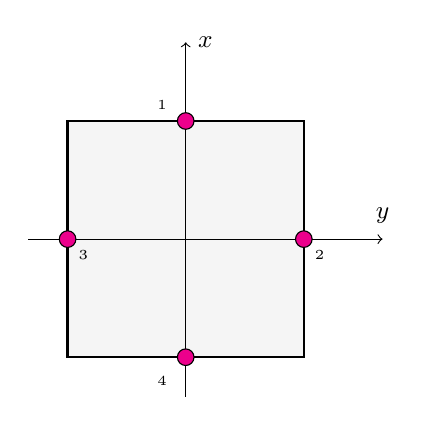
\begin{tikzpicture}
%\draw[step=1cm,gray,very thin] (0,0) grid (8,8); %background grid

\draw[thick,fill=gray!8] (1,1) -- (4,1) -- (4,4) -- (1,4) -- cycle;

\node[] at (1.2,2.3) {\tiny 3};
\node[] at (4.2,2.3) {\tiny 2};
\node[] at (2.2,.7) {\tiny 4};
\node[] at (2.2,4.2) {\tiny 1};

\draw[->] (0.5,2.5)--(5,2.5);
\draw[->] (2.5,0.5)--(2.5,5);

\draw[black,fill=magenta] (1,2.5)   circle (3pt);
\draw[black,fill=magenta] (4,2.5)   circle (3pt);
\draw[black,fill=magenta] (2.5,1)   circle (3pt);
\draw[black,fill=magenta] (2.5,4)   circle (3pt);

\node[] at (5,2.8) {\small $y$};
\node[] at (2.75,5) {\small $x$};
\end{tikzpicture}
\end{center}




\begin{verbatim}
+======3======+
|             |
|      s      |
|      |      |
4      +--r   2
|             |
|             |
|             |
+======1======+
\end{verbatim}

There are two types of basis functions: the Middle Point (MP) variant
such that $\bN_i(\vec{r}_j)=\delta_{ij}$ and the Mid Value (MV) variant
such that $\frac{1}{|\Gamma_i|} \int_{\Gamma_i} \bN_j d\Gamma = \delta_{ij}$.

%.............................................
\paragraph{The Middle Point (MP) variant}. 
We have $\tilde{Q}_1=span \{ 1,r,s,r^2-s^2 \}$
so a function $f \in \tilde{Q}_1$  is such that 
\begin{equation}
f(r,s)= a + b r + c s + d(r^2-s^2 )
\label{nonpsf}
\end{equation}
This function must be so that 
\begin{eqnarray}
f_1 &=& f(r=0 ,s=-1) = a -c -d \\
f_2 &=& f(r=+1,s=0)  = a +b +d \\
f_3 &=& f(r=0 ,s=+1) = a +c -d \\
f_4 &=& f(r=-1,s=0)  = a -b +d 
\end{eqnarray}
and then 
\[
\left(
\begin{array}{c}
f_1 \\ f_2 \\ f_3 \\ f_4
\end{array}
\right)
=
\left(
\begin{array}{cccc}
1 &0 &-1 &-1 \\
1 &1 &0 &1 \\
1 &0 &1 &-1 \\
1 &-1 &0 &1
\end{array}
\right)
\cdot
\left(
\begin{array}{c}
a \\ b \\ c \\ d
\end{array}
\right)
\]
This system can easily be solved, and $a,b,c,d$ are then replaced in Eq.~\eqref{nonpsf},
which yields 
\begin{eqnarray}
f(r,s) &=& \bN_1(r,s)f_1 +\bN_2(r,s)f_2 + \bN_3(r,s)f_3 +\bN_4(r,s)f_4
\end{eqnarray}
inside the element with
\begin{mdframed}[backgroundcolor=blue!5]
\begin{eqnarray}
\bN_1(r,s) &=& \frac{1}{4} (1-2s-(r^2-s^2)) \nonumber\\
\bN_2(r,s) &=& \frac{1}{4} (1+2r+(r^2-s^2)) \nonumber\\
\bN_3(r,s) &=& \frac{1}{4} (1+2s-(r^2-s^2)) \nonumber\\
\bN_4(r,s) &=& \frac{1}{4} (1-2r+(r^2-s^2)) \nonumber
\end{eqnarray}
\end{mdframed}
We of course recover the partition of unity property, i.e. $\sum \bN_i(r,s)=1$ for any coordinate $r,s$ inside 
the reference element.

\begin{remark}
These basis functions have been independently proposed by \textcite{dogm81} (1981). The authors
prove herein that this element is checkerboard-free (although they do no show any example
of simulation carried out with this element).
\end{remark}

\begin{eqnarray}
\frac{\partial \bN_1}{\partial r} &=& \frac{1}{2}(-r)\\
\frac{\partial \bN_2}{\partial r} &=& \frac{1}{2}(1+r)\\
\frac{\partial \bN_3}{\partial r} &=& \frac{1}{2}(-r)\\
\frac{\partial \bN_4}{\partial r} &=& \frac{1}{2}(-1+r)
\end{eqnarray}

\begin{eqnarray}
\frac{\partial \bN_1}{\partial s} &=& \frac{1}{2}(-1+s)\\
\frac{\partial \bN_2}{\partial s} &=& \frac{1}{2}(-s)\\
\frac{\partial \bN_3}{\partial s} &=& \frac{1}{2}(1+s)\\
\frac{\partial \bN_4}{\partial s} &=& \frac{1}{2}(-s)
\end{eqnarray}

\begin{center}
\includegraphics[width=6cm]{images/rannacherturek/N1}
\includegraphics[width=6cm]{images/rannacherturek/N2}\\
\includegraphics[width=6cm]{images/rannacherturek/N3}
\includegraphics[width=6cm]{images/rannacherturek/N4}\\
{\captionfont Graphical representation of the $\tilde{Q}_1$ basis functions}
\end{center}

%......................................
\paragraph{The Mid Value (MV) variant}. 

These basis functions are implemented in deal.II
\footnote{\url{https://www.dealii.org/8.5.0/doxygen/deal.II/polynomials_rannacher_turek_8cc_source.html}}
for $x\in[0,1]$ and $y\in[0,1]$:

\begin{eqnarray}
\bN_1(x,y) &=&  0.75 + 1.5x - 2.5y -1.5(x^2-y^2) \quad bottom\\
\bN_2(x,y) &=& -0.25 - 0.5x + 1.5y +1.5(x^2-y^2) \quad right\\
\bN_3(x,y) &=& -0.25 + 1.5x - 0.5y -1.5(x^2-y^2) \quad top\\
\bN_4(x,y) &=&  0.75 - 2.5x + 1.5y +1.5(x^2-y^2) \quad left
\end{eqnarray}
We then proceed to rewrite these for $r\in[-1,1]$ and $t\in[-1:1]$:
\begin{mdframed}[backgroundcolor=blue!5]
\begin{eqnarray}
\bN_1(r,s) &=& \frac{1}{4} -\frac{1}{2}s - \frac{3}{8}(r^2-s^2) \quad bottom \\
\bN_2(r,s) &=& \frac{1}{4} +\frac{1}{2}r + \frac{3}{8}(r^2-s^2) \quad right \\
\bN_3(r,s) &=& \frac{1}{4} +\frac{1}{2}s - \frac{3}{8}(r^2-s^2) \quad top \\
\bN_4(r,s) &=& \frac{1}{4} -\frac{1}{2}r + \frac{3}{8}(r^2-s^2) \quad left
\end{eqnarray}
\end{mdframed}
It is easy to verify that these functions verify the property
\[
\frac{1}{|\Gamma_i|} \int_{\Gamma_i} N_j d\Gamma = \delta_{ij}
\]
These basis functions are used in Shipeng \& Zhongci (2006) \cite{shzh06} 
and mentioned in John \cite[p.722]{john16}.
\begin{eqnarray}
\frac{\partial N_1}{\partial r} &=& -\frac{3}{4}r \nonumber\\
\frac{\partial N_2}{\partial r} &=& \frac{1}{2}+\frac{3}{4}r \nonumber\\
\frac{\partial N_3}{\partial r} &=& -\frac{3}{4}r \nonumber\\
\frac{\partial N_4}{\partial r} &=& -\frac{1}{2}+\frac{3}{4}r \nonumber
\end{eqnarray}

\begin{eqnarray}
\frac{\partial N_1}{\partial t} &=& -\frac{1}{2}+\frac{3}{4}t \nonumber\\
\frac{\partial N_2}{\partial t} &=& -\frac{3}{4}t \nonumber\\
\frac{\partial N_3}{\partial t} &=& \frac{1}{2}+\frac{3}{4}t \nonumber\\
\frac{\partial N_4}{\partial t} &=& -\frac{3}{4}t \nonumber
\end{eqnarray}

